\section{Experimental Results}
\label{sec:4_5_Expsetup}

The experiments conducted in this study were designed to assess the effect of concept drift on the performance of the proposed framework in detecting emerging new classes. The primary goal was to identify the machine learning algorithm in conjunction with the Dynamic Ensemble Selection (DES) technique, which improves classification accuracy and robustness when faced with the emergence of new classes. By conducting these experiments, valuable insights were gained, leading to potential enhancements in the performance of the proposed approach and its ability to handle imbalanced data streams effectively. The findings of these experiments contribute to a better understanding of the framework's capabilities and shed light on the optimal approach for handling emerging new classes in the presence of concept drift. The results provide valuable guidance for selecting the most suitable classification machine learning algorithm and DES configuration to improve the classification accuracy and robustness. The experiments conducted in this study provide valuable insights into enhancing the performance of the proposed approach and effectively addressing the challenges posed by emerging new classes and concept drifts in the incremental drifted streams. These insights can contribute to advancing stream mining techniques and developing more accurate and robust classification models in dynamic and evolving data stream environments. The two main questions to be answered are:

\begin{itemize}
  \setlength{\itemindent}{-.5in}
  
      \item $\pmb{Q_1}$: How does the emergence of new classes in data streams affect the stability and performance of ML models?
      \item  $\pmb{Q_2}$: how can ML models be adapted to accommodate such changes?
  \end{itemize}

\subsection{Experimental setup}
The evaluation of the proposed approach involves a comparison with SENCForest \cite{mu2017classification}, SENNE \cite{yang2021concept}, and KENNES \cite{zhang2022knnens} which employs multiple metrics such as precision, recall, F1 score \cite{sasaki2007truth}, BAC \cite{brodersen2010balanced}, and G-mean \cite{kubat1997addressing}. The experimental protocol employed for evaluation followed the test-then-train approach \cite{krawczyk2017ensemble}, where the classification model is trained on a specific data chunk and subsequently evaluated on the next chunk. The chunk size was standardized to 2000 instances. Four different classification models were used as base estimators: K-Nearest Neighbors (KNN) algorithm, Support Vector classifier (abbreviated as SVC), Gaussian Naive Bayes abbreviated as (GNB), and Hoeffding Tree (abbreviated as HT), as implemented in scikit-learn \cite{ksieniewicz2022stream}. We establish an ensemble classifier pool with a set limit of L = 8, wherein each ensemble consists of N = 4 base models. While these constraints remained fixed across all our experiments, the threshold for the pool classifier in each approach was maintained at eight. Consequently, if the threshold is surpassed, the least-performing classifier is systematically eliminated. ADWIN \cite{adams2023explainable} and DDM \cite{gama2004learning} are employed as concept drift detectors as implemented in the River library , to identify concept drifts, as they are considered more accurate techniques for use in incremental data streams \cite{gama2004learning}\cite{adams2023explainable}\cite{madkour2023historical}\cite{baena2006early}. This configuration was applied consistently across all approaches to ensure fair engagement. The experiments were carried out using the Python programming language, with the source code publicly accessible on GitHub . 
\subsection{Data Streams}
In this study, the performance of the proposed approach was evaluated using various datasets, including synthetic data streams, a real application stream, and dataset benchmark datasets. To conduct the evaluations, the stream-learn and River python libraries \cite{ksieniewicz2022stream} were used. As detailed in Table \ref{tab:5_1}, the benchmark dataset employed in the study is the Covertype dataset stream. This dataset comprises 52 features, 7 classes, and a total of 581,010 instances. It serves as a standard benchmark dataset widely used in stream mining research. For the evaluation of real application streams, the Sensor stream dataset was utilized. This dataset includes 5 features, 58 classes, and a total of 392,600 instances, representing a real-world application scenario. Synthetic dataset stream was generated using the scikit-learn Python package \cite{ksieniewicz2022stream}. This synthetic dataset was created to simulate data streams and evaluate the performance of the proposed approach. The synthetic datasets consisted of 10 features and four classes and were divided into 200 chunks. Each chunk had a size of 2,000. The performance of the proposed approach was systematically evaluated using these datasets and a stream-learn library. These evaluations provided valuable insights into the effectiveness of the approach in handling different types of data streams, including benchmark datasets, real application streams, and synthetic data streams.
\begin{table}[!ht]
  \centering
  \begin{tabular}{|c|c|c|c|}
  \hline
  \textbf{Dataset} & \textbf{Number of Features} & \textbf{Number of Classes} & \textbf{Number of Instances} \\ \hline
  Covertype dataset$^2$ & 52 & 7 & 581,010  \\ \hline
  Sensor Stream dataset$^3$ & 5 & 58 & 392,600 \\ \hline
  Synthetic stream & 8 & 3 & 200,000 \\ \hline
  \end{tabular}
  \caption{Characteristics of the datasets used in the experimentation.}
  \label{tab:5_1}
  \end{table}

\subsection{COMPARED APPROACHES}
In the following section, we present a comparative analysis between our proposed GNB methodology and three established benchmark techniques, detailed as follows:
\begin{itemize}
  \item \textbf{SENCForest \cite{mu2017classification}:} The SENCForest method, which uses anomaly detection techniques for new class identification, is based on completely random trees. It subsamples from each class to build isolation trees for both classification and detection, using 20 random trees and a subsample size of 20. Despite its ability to function with partial or no label information, it often encounters high false positive rates and inefficiency in runtime performance in practical scenarios.
  \item \textbf{SENNE \cite{zhu2020semi}:} Utilizing a hypersphere ensemble mechanism, SENNE calculates scores to identify both new and known classes. It operates with a buffer capacity of 100 and sets a new class-score threshold of 0.5.
  \item  \textbf{KENNES \cite{zhang2022knnens}:} The KNNENS method addresses the dual challenge of detecting new classes and classifying known classes within a unified framework. It was configured with a buffer size of 100 and a new class score threshold of 0.5.
\end{itemize}
\subsection{Analysis of Experimental Results}
This section presents a comprehensive evaluation of the performance of the proposed approach (PA) across multiple data streams. To guarantee a thorough assessment, five performance metrics—F1 score, precision, recall, G-mean, and BAG—were presented using two visualization diagrams: radar and line. A radar chart was cleverly utilized to provide a comprehensive summary, precisely demonstrating the performance of each algorithm across the six key metrics. To assess the overall performance of each approach—namely, the PA, SENCForest, SENNE, and KENNES—the average value of each metric was calculated. Additionally, a line diagram using the G-mean metric was used to compare these methods for each chunk across 200 chunks. A radar diagram provided a detailed and nuanced evaluation of the proposed approach’s performance across various experimental scenarios.
\subsubsection{Results on the Benchmark Stream}
This experiment focused on assessing the accuracy of SENCForest, SENNE, KENNES, and PA across 200 chunks of a sensor data stream, utilizing varying buffer sizes similar to the previous experiment. The results, shown in Fig. \ref{fig:5_resul1}, were visualized using scatter plots. Fig. \ref{fig:5_result1} (a) displays the classification accuracy for each algorithm with a buffer size of 5. The PA algorithm achieved the highest performance overall, except for chunks 43 to 48, where some instances were incorrectly assumed as outliers rather than emergent. In contrast, SENCForest and SENNE had the lowest accuracy. Additional experiments with buffer sizes of 10 and 20 (Fig. \ref{fig:5_result1}(b) and Fig. \ref{fig:5_result1}(c)) demonstrated reduced accuracy compared to the buffer size of 5, attributed to fewer updates with larger buffer sizes. The adaptive buffer size experiment in Fig. \ref{fig:5_result1}(d) reaffirmed the effectiveness of the PA algorithm, which outperformed others across all chunks, with the adaptive emerging pool size providing optimal results.

\begin{figure}[!ht]
	\centering
	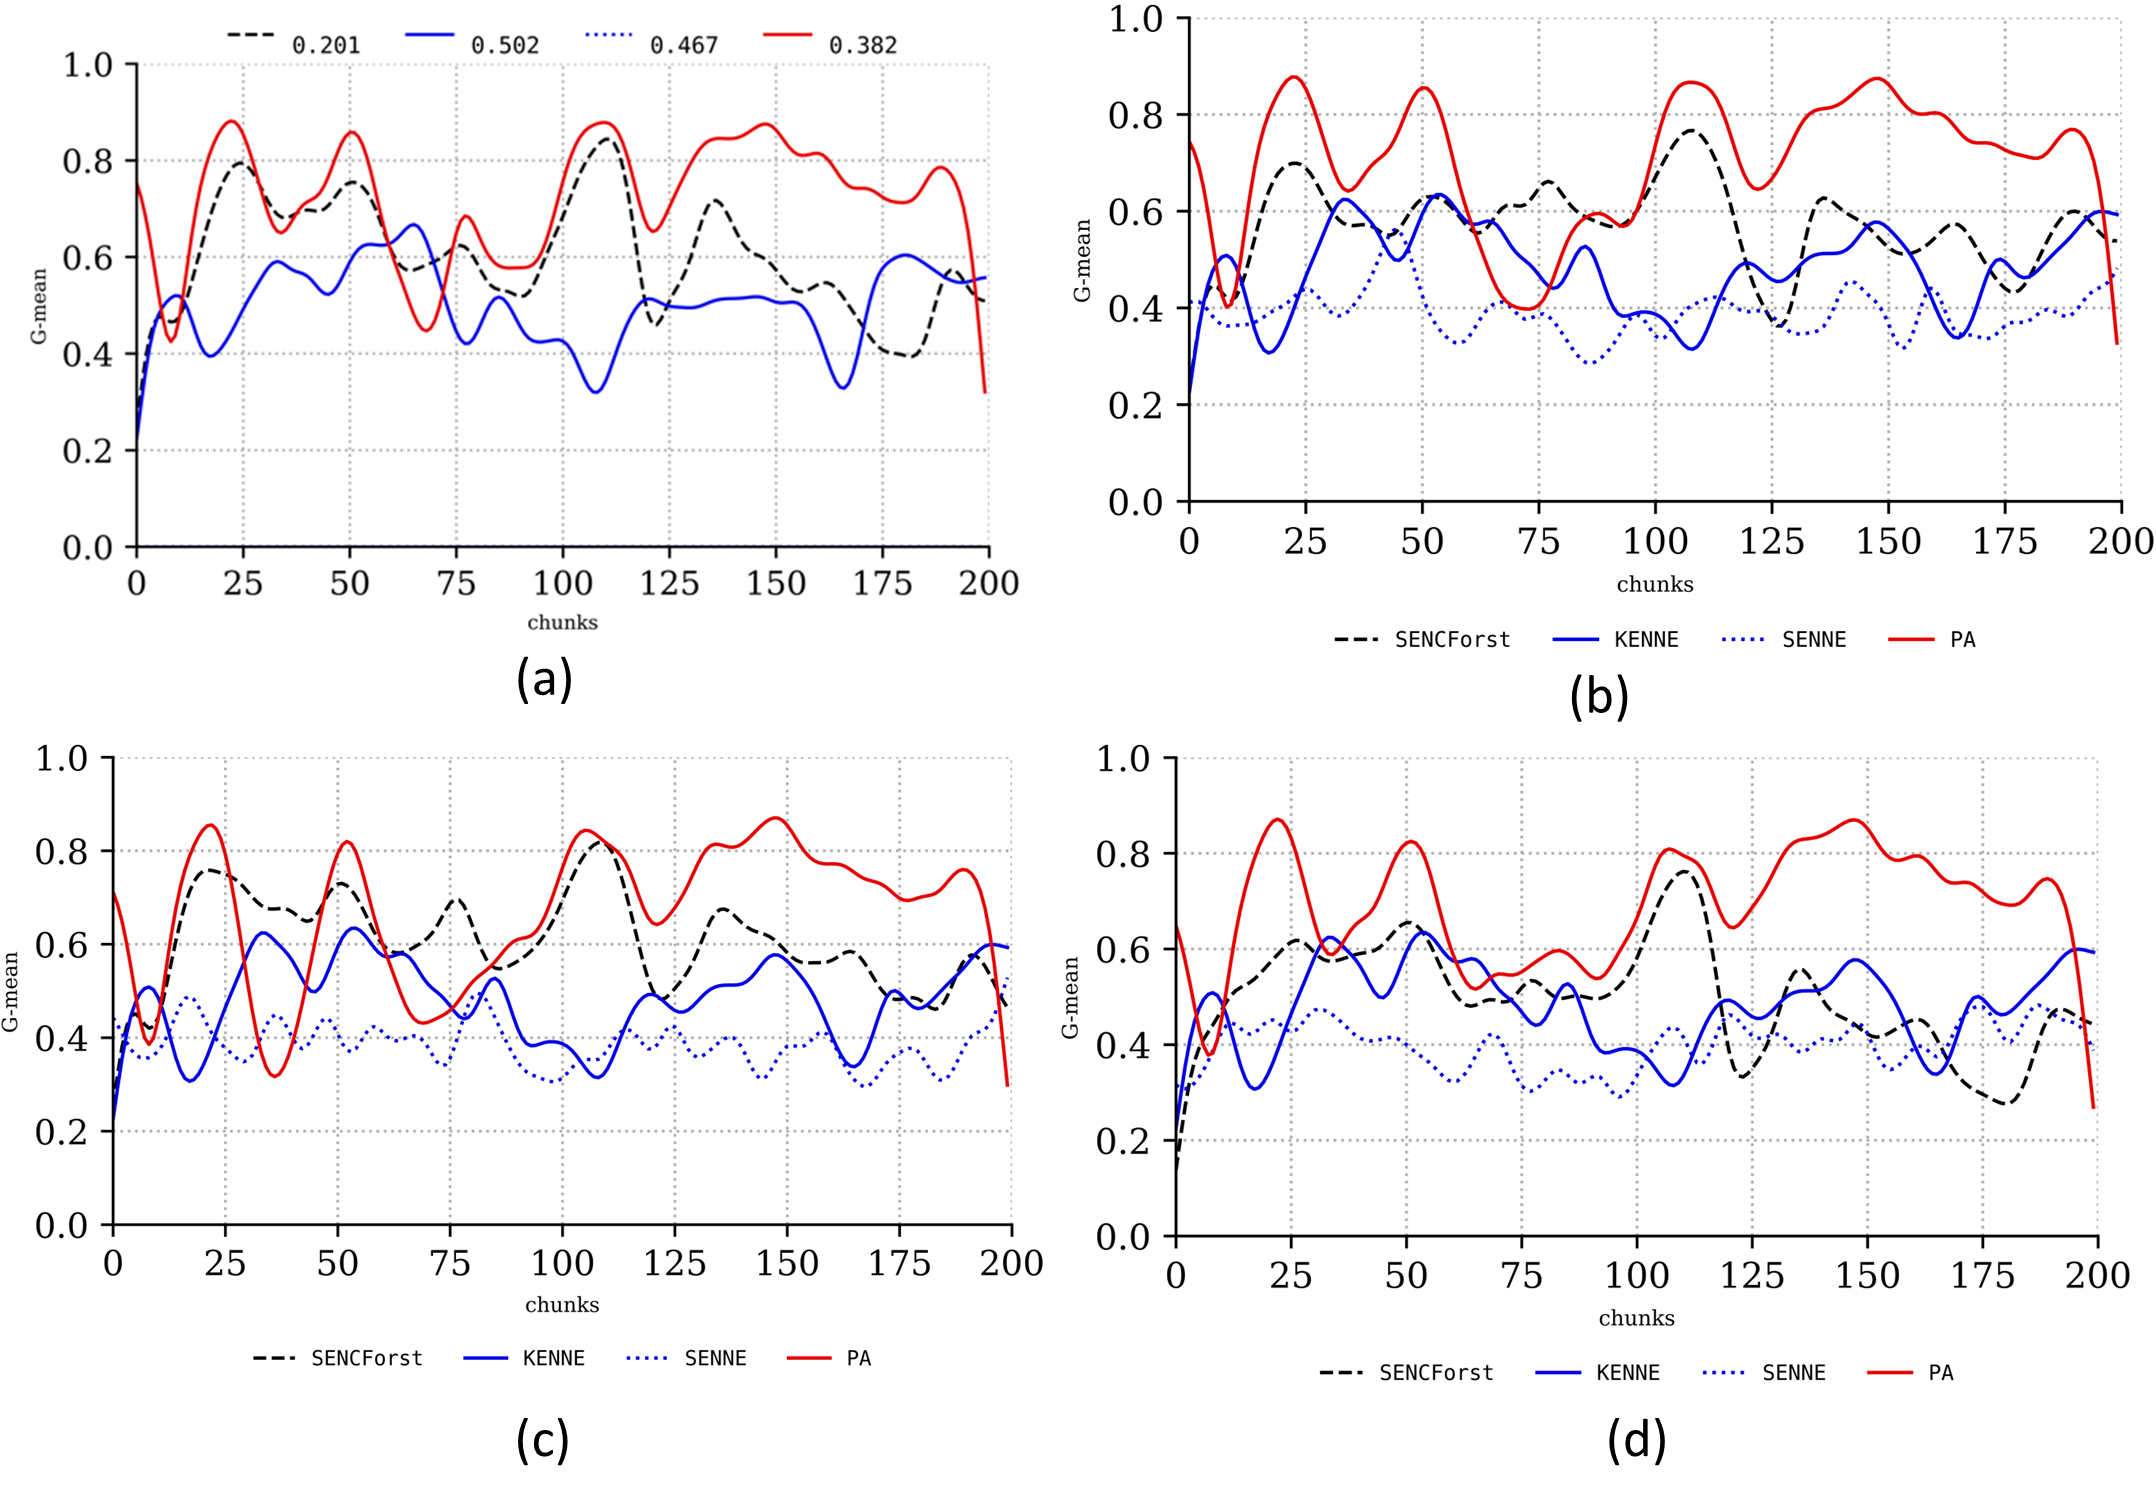
\includegraphics[width=1\linewidth]{5_Emerging/figures/result1}
	\caption{Covertype stream for various emerging buffer sizes: (a) buffer size of 5, (b) buffer size of 10, (c) buffer size of 20, and (d) our adaptive buffer size.}
	\label{fig:5_result1}
\end{figure}

\subsubsection{Results on the Real Application Stream}
This experiment focused on assessing the accuracy of SENCForest, SENNE, KENNES, and PA across 200 chunks of a sensor data stream, utilizing varying buffer sizes similar to the previous experiment. The results, shown in Fig. \ref{fig:5_result2}, were visualized using scatter plots. Fig. \ref{fig:5_result2}(a) displays the classification accuracy for each algorithm with a buffer size of 5. The PA algorithm achieved the highest performance overall, except for chunks 43 to 48, where some instances were incorrectly assumed as outliers rather than emergent. In contrast, SENCForest and SENNE had the lowest accuracy. Additional experiments with buffer sizes of 10 and 20 (Fig. \ref{fig:5_result2}(b) and Fig. \ref{fig:5_result2}(c)) demonstrated reduced accuracy compared to the buffer size of 5, attributed to fewer updates with larger buffer sizes. The adaptive buffer size experiment in Fig. \ref{fig:5_result2}(d) reaffirmed the effectiveness of the PA algorithm, which outperformed others across all chunks, with the adaptive emerging pool size providing optimal results.

\begin{figure}[!ht]
	\centering
	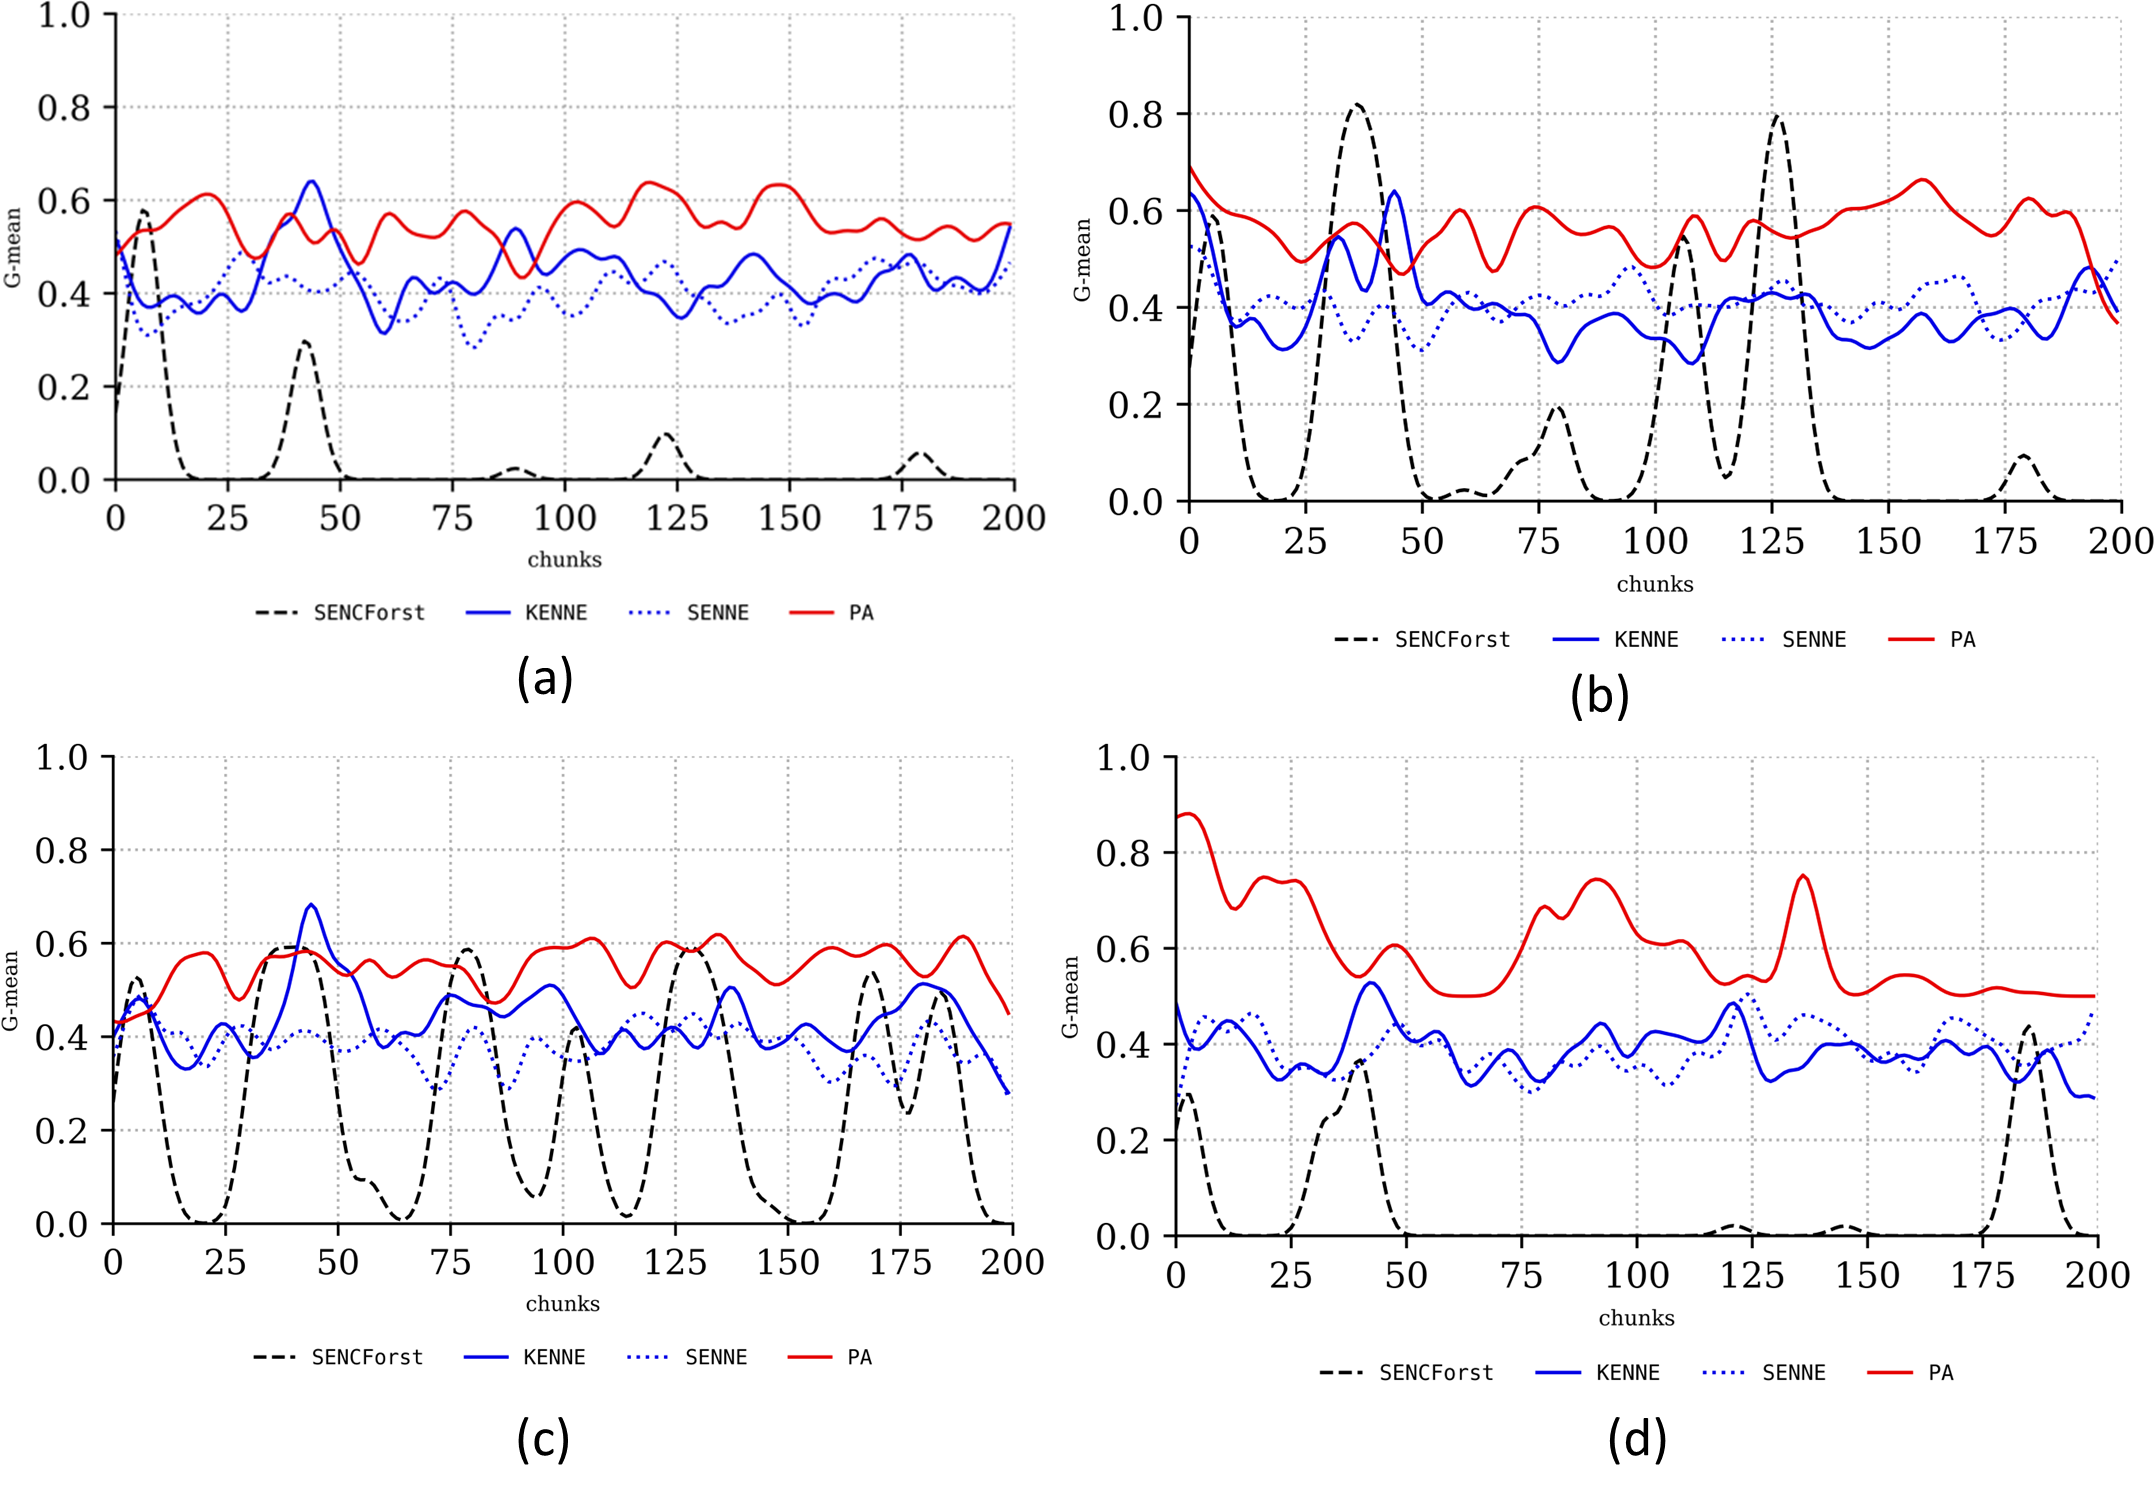
\includegraphics[width=1\linewidth]{5_Emerging/figures/result2}
	\caption{Sensor stream for various emerging buffer sizes: (a) buffer size of 5, (b) buffer size of 10, (c) buffer size of 20, and (d) our adaptive buffer size.}
	\label{fig:5_result2}
\end{figure}

\subsubsection{Results on the Synthetic Stream}
This experiment aimed to assess the performance of the previously tested methods on a synthetic data stream. Results, depicted in Fig. \ref{fig:5_result3}, were analyzed using radar and scatter plots. Fig. \ref{fig:5_result2}(a) shows the performance of various algorithms using a buffer size of 5, with the radar plot highlighting PA's superior performance. Scatter plots illustrate that PA consistently delivered the highest accuracy when applied to the synthetic stream with buffer sizes of 5, 10, and 20, as shown in Fig. \ref{fig:5_result3}(a), Fig. \ref{fig:5_result3}(b), and Fig. \ref{fig:5_result3}(c), respectively. Fig. \ref{fig:5_result3}(d) demonstrates that the adaptive pool size yielded the best accuracy on the synthetic stream, underscoring the adaptability and efficiency of the PA algorithm.

\begin{figure}[!ht]
	\centering
	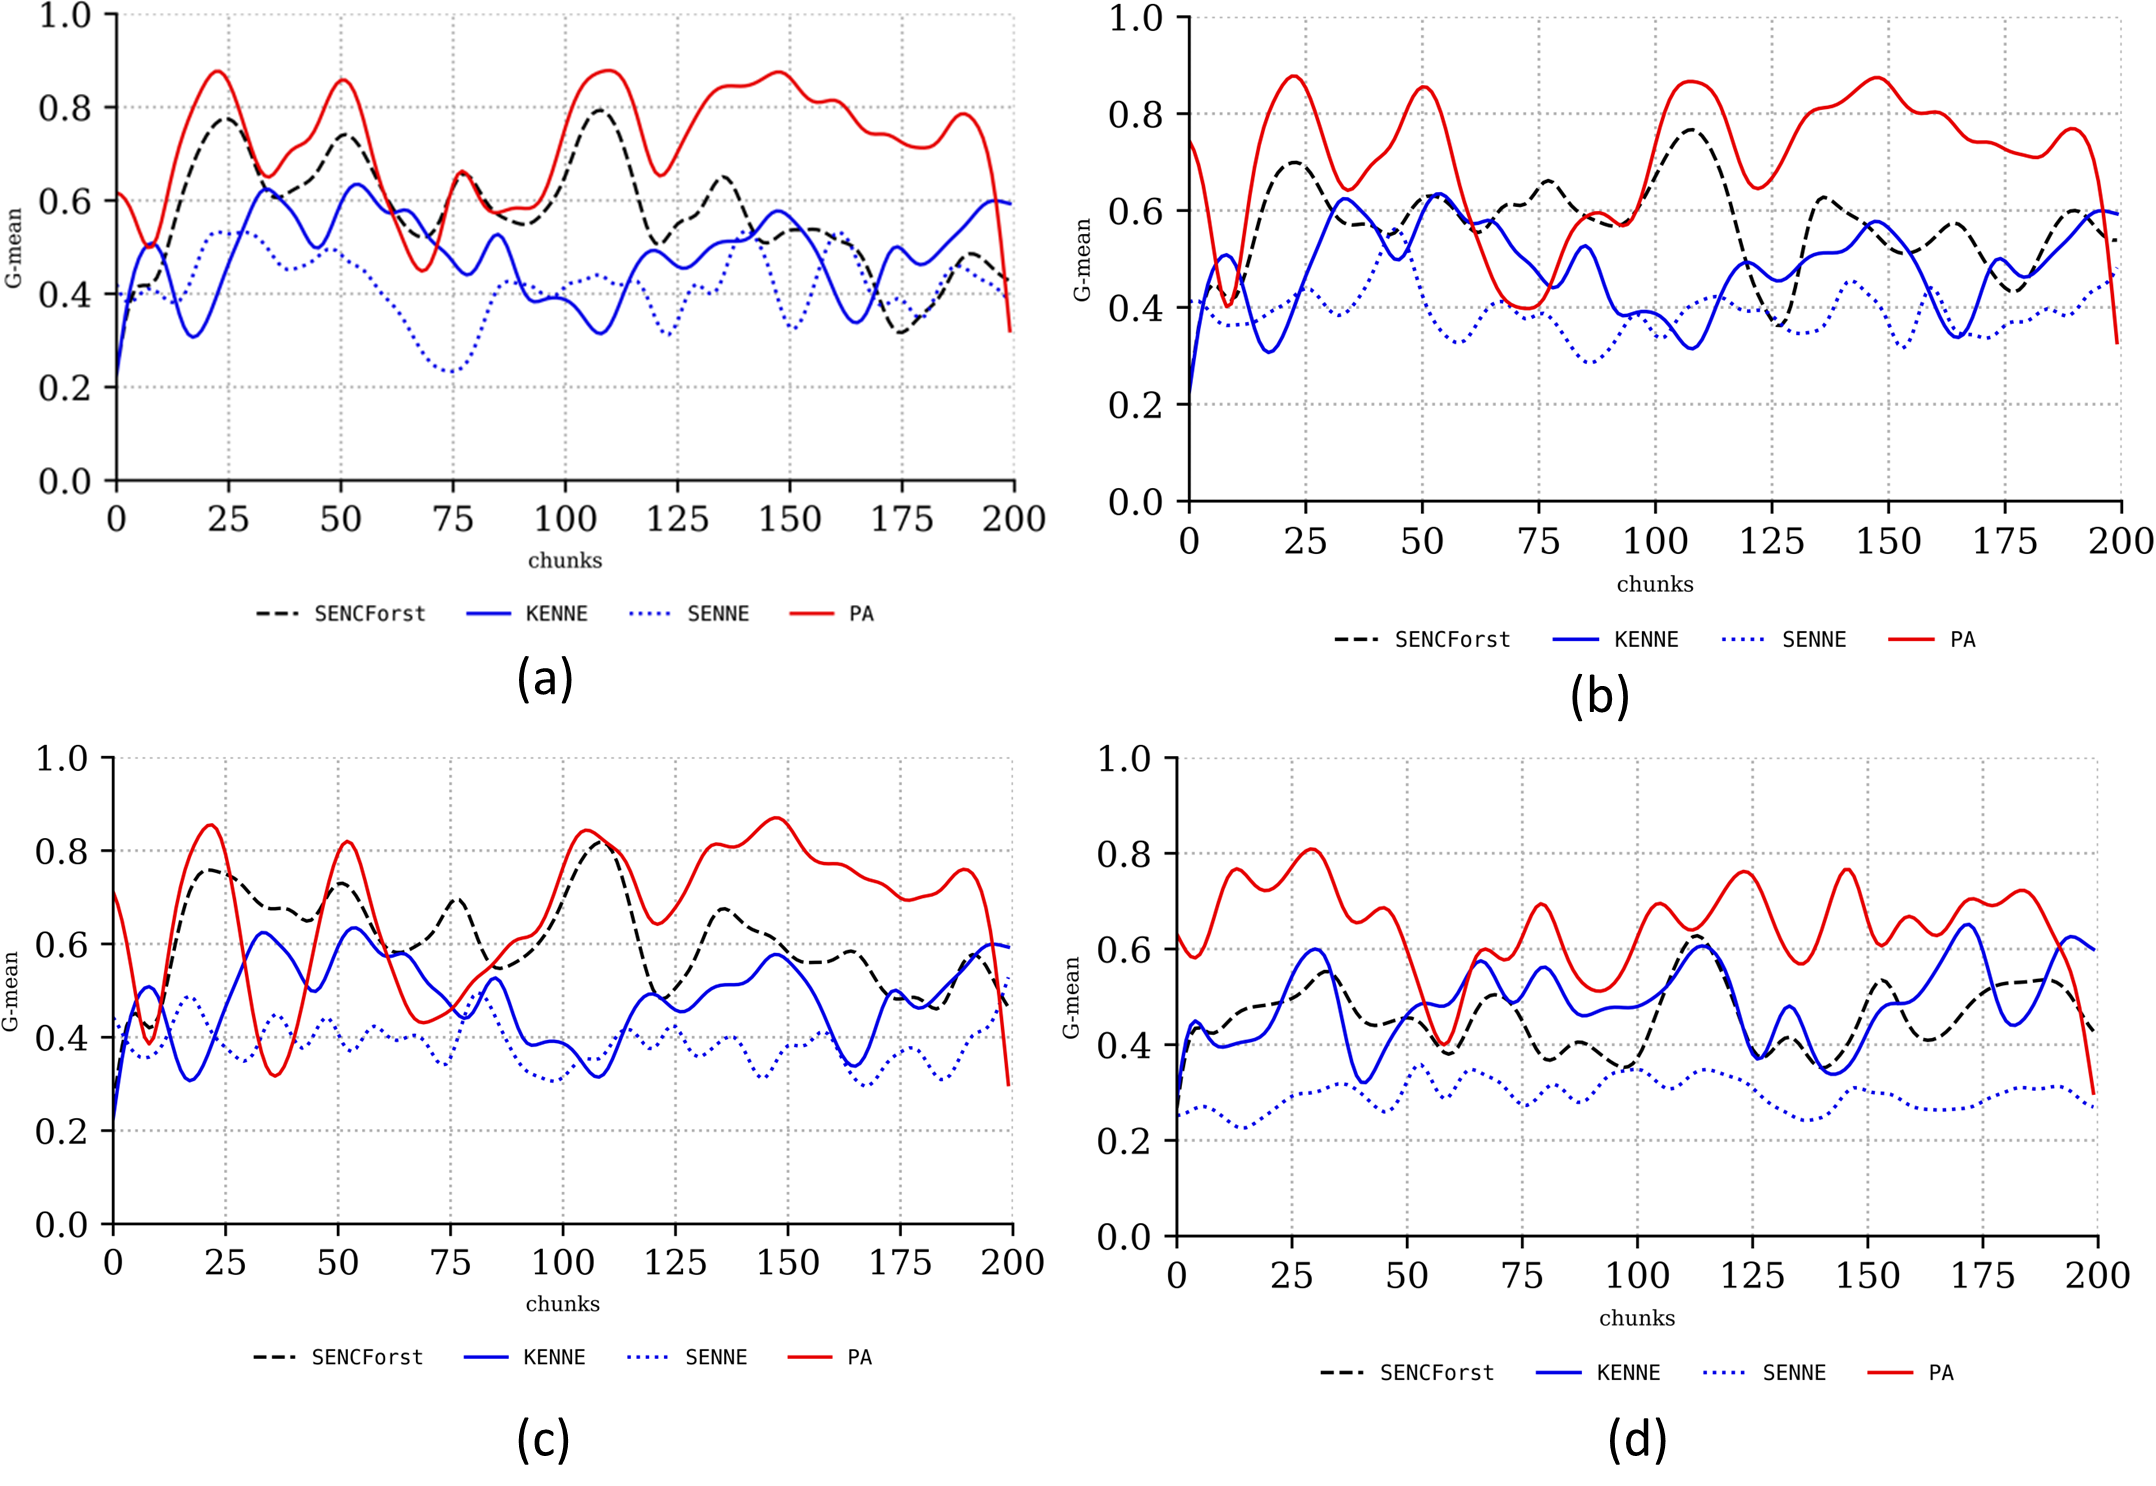
\includegraphics[width=1\linewidth]{5_Emerging/figures/result3}
	\caption{Synthetic stream for various emerging buffer sizes: (a) buffer size of 5, (b) buffer size of 10, (c) buffer size of 20, and (d) our adaptive buffer size.}
	\label{fig:5_result3}
\end{figure}

\subsection{Runtime analysis of the best algorithms}
Our experimental results revealed that selecting the optimal algorithm for detecting emerging new classes is influenced by various factors, including dataset characteristics, buffer length, and the algorithm's runtime requirements. We conducted a series of experiments to evaluate the runtime performance of different algorithms and observed that the PA algorithm demonstrated outstanding efficiency. Specifically, with the adaptive pool size approach, the PA algorithm trained bagging classifiers 150 times within 2131 seconds when using the Covertype stream, outperforming others despite SENCForest achieving the lowest runtime but with fewer updates compared to PA as shown in Table \ref{tab:5_1}. On the Sensor stream, PA delivered the best runtime for 66 updates, while SENCForest, KENNES, and SENNE required more time to complete the same or fewer iterations. Similarly, PA exhibited superior runtime performance on the Synthetic stream. These results underscore the PA algorithm’s efficiency, making it an ideal choice for time-constrained scenarios. The superior runtime performance of PA is further highlighted in bold in Table \ref{tab:5_1}.
\begin{table}[!ht]
  \centering
  \caption{Running Time of SENCForest, SENNE, KENNES, and PA}
  \label{table:5_2}
  \begin{tabular}{|c|c|c|c|}
  \hline
  \textbf{Stream}  & \textbf{Algorithm} & \textbf{Training Times} & \textbf{Time (seconds)} \\ \hline
  \textbf{Covertype} & SENCForest & 142 & 1997 \\ \cline{2-4} 
   & SENNE & 5 & 2167 \\ \cline{2-4} 
   & KENNES & 3 & 1742 \\ \cline{2-4} 
   & PA & 150 & 2131 \\ \hline
  \textbf{Sensor} & SENCForest & 23 & 1244 \\ \cline{2-4} 
   & SENNE & 17 & 3825 \\ \cline{2-4} 
   & KENNES & 152 & 2109 \\ \cline{2-4} 
   & PA & 66 & 1075 \\ \hline
  \textbf{Synthetic} & SENCForest & 12 & 107 \\ \cline{2-4} 
   & SENNE & 26 & 224 \\ \cline{2-4} 
   & KENNES & 149 & 2022 \\ \cline{2-4} 
   & PA & 47 & 91 \\ \hline
  \end{tabular}
  \end{table}
  \subsection{Comparison between GNB, KNN, and HT, SVC as a base classifier}
  In this section, we compare various algorithms (KNN, SVC, GNB, and HT) as base classifiers for the bagging technique. The comparison, illustrated in Fig. \ref{fig:5_result4}, focuses on the Covertype dataset stream, where GNB (blue line) and HT (red line) consistently achieve the highest scores across most chunks. Both classifiers also excel in radar plots across key performance metrics, including accuracy, precision, recall, and F1-score. Based on these results, GNB and HT emerge as the most suitable base classifiers for the bagging technique. We further compared GNB and HT in terms of runtime and update frequency, as shown in Table \ref{table:5_3}. The results indicate that GNB has the best runtime performance, while HT demonstrates superior accuracy, likely due to its higher number of updates compared to GNB, as reflected in Table 3 and Fig. \ref{fig:5_result4}.
  \begin{figure}[!ht]
    \centering
    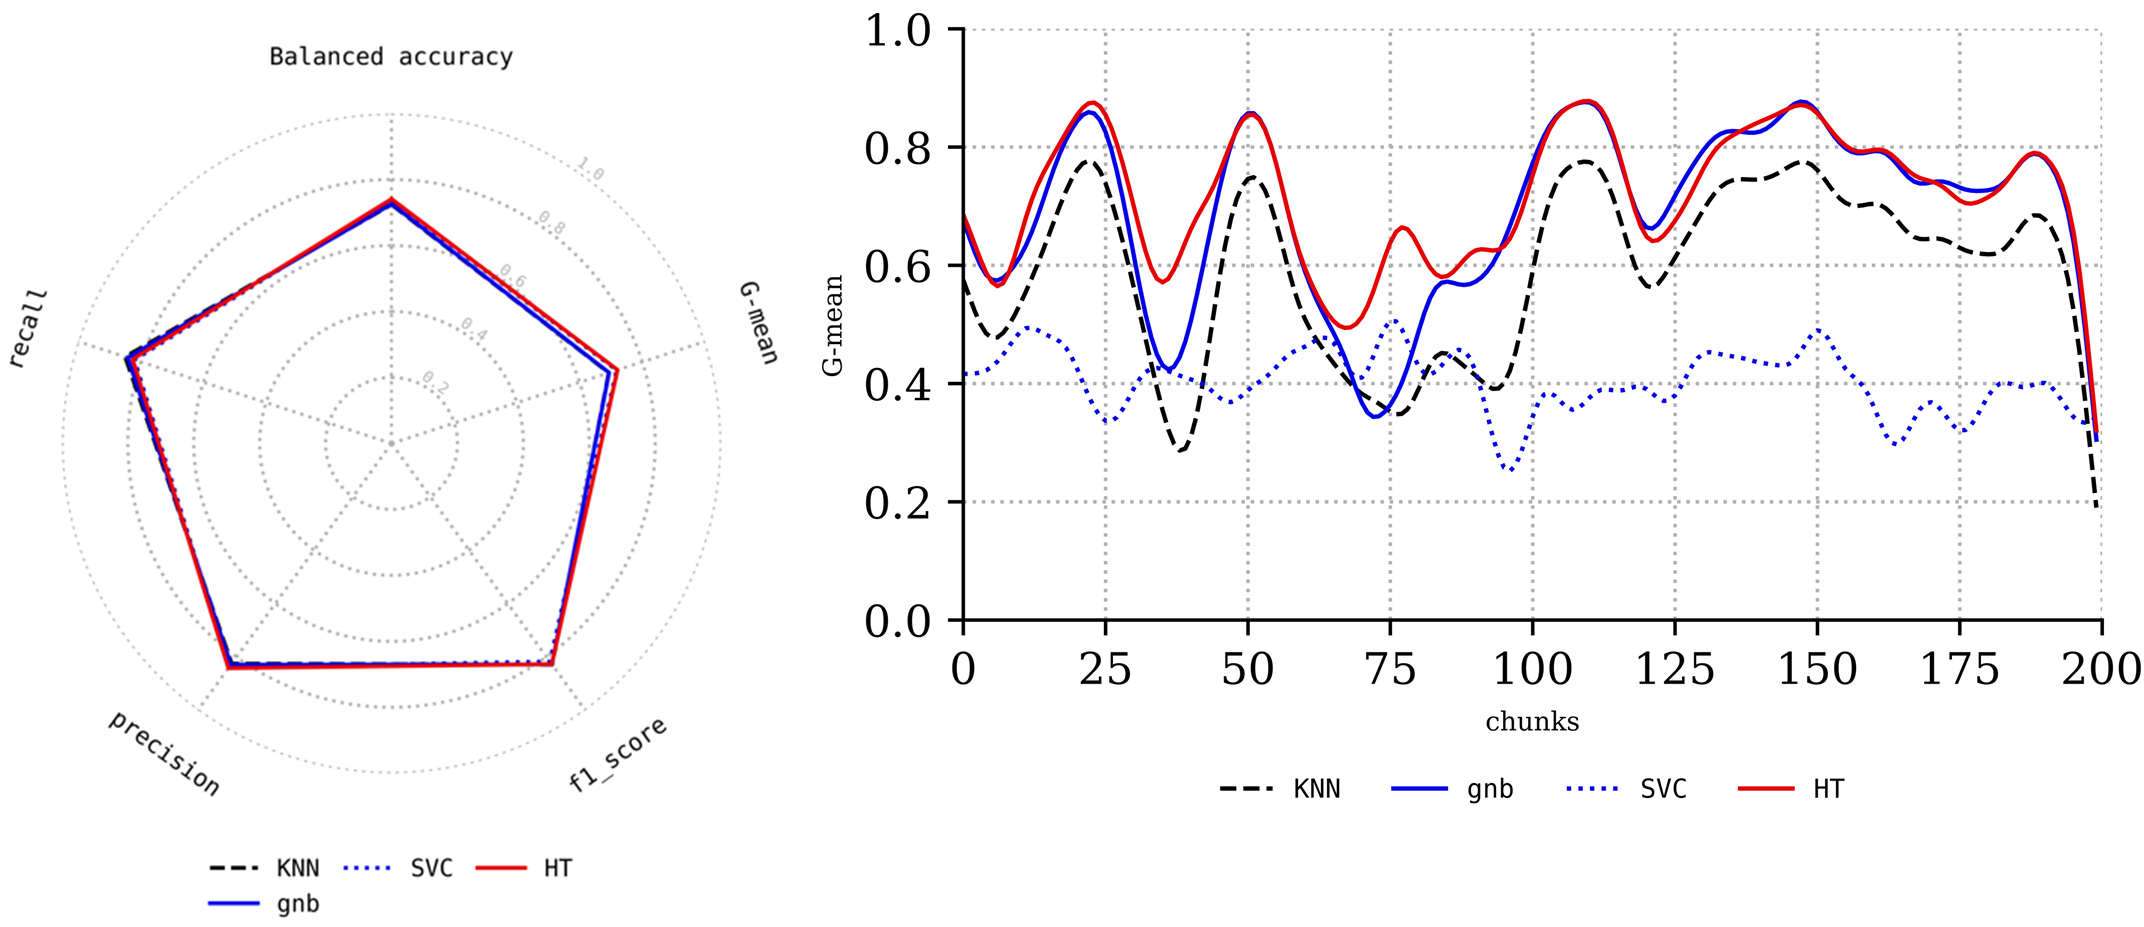
\includegraphics[width=1\linewidth]{5_Emerging/figures/result4}
    \caption{Covertype stream for concept drift detector (ADWIN, DDM) via several metrics (recall, precision, balanced accuracy, G-mean, and f1-score)}
    \label{fig:5_result4}
  \end{figure}

  \begin{table}[h!]
    \centering
    \caption{Running time comparsion between GNB, KNN, and HT, SVC as a base classifier}
      \label{table:5_3}
    \begin{tabular}{|c|c|c|c|c|}
      
    \hline
    \textbf{Algorithm} & \textbf{KNN} & \textbf{SVC} & \textbf{GNB} & \textbf{HT} \\ \hline
    \textbf{Training Times} & 140 & 150 & 139 & 148 \\ \hline
    \textbf{Time (seconds)} & 586 & 878 & \textbf{291} & 1169 \\ \hline
    \end{tabular}
    \end{table}

    \subsection{Running time and accuracy comparsions between ADWIN and DDM}
    In this section, we compare two concept drift detection methods: the Drift Detection Method (DDM) \cite{gama2004learning} and the Adaptive Window (ADWIN) \cite{gama2004learning}\cite{adams2023explainable}. These methods are widely recognized for their excellent performance in handling incremental drifted streams \cite{gama2004learning}\cite{adams2023explainable}\cite{madkour2023historical}\cite{baena2006early}. As shown in Fig. \ref{fig:5_result5}, using the Covertype stream with GNB as the base classifier, ADWIN consistently outperforms DDM in both radar and line plots across all performance metrics, including accuracy. Furthermore, when comparing their runtime and update frequency, as presented in Table \ref{table:5_4}, ADWIN proves to be the superior detector for drifted streams. It identifies the highest number of drifts (139) in the least amount of time (272 seconds), demonstrating its efficiency and effectiveness.

    \begin{figure}[!ht]
      \caption{Covertype stream for concept drift detector (ADWIN, DDM) via several metrics (recall, precision, balanced accuracy, G-mean, and f1-score)}
      \label{fig:5_result5}
      \centering
      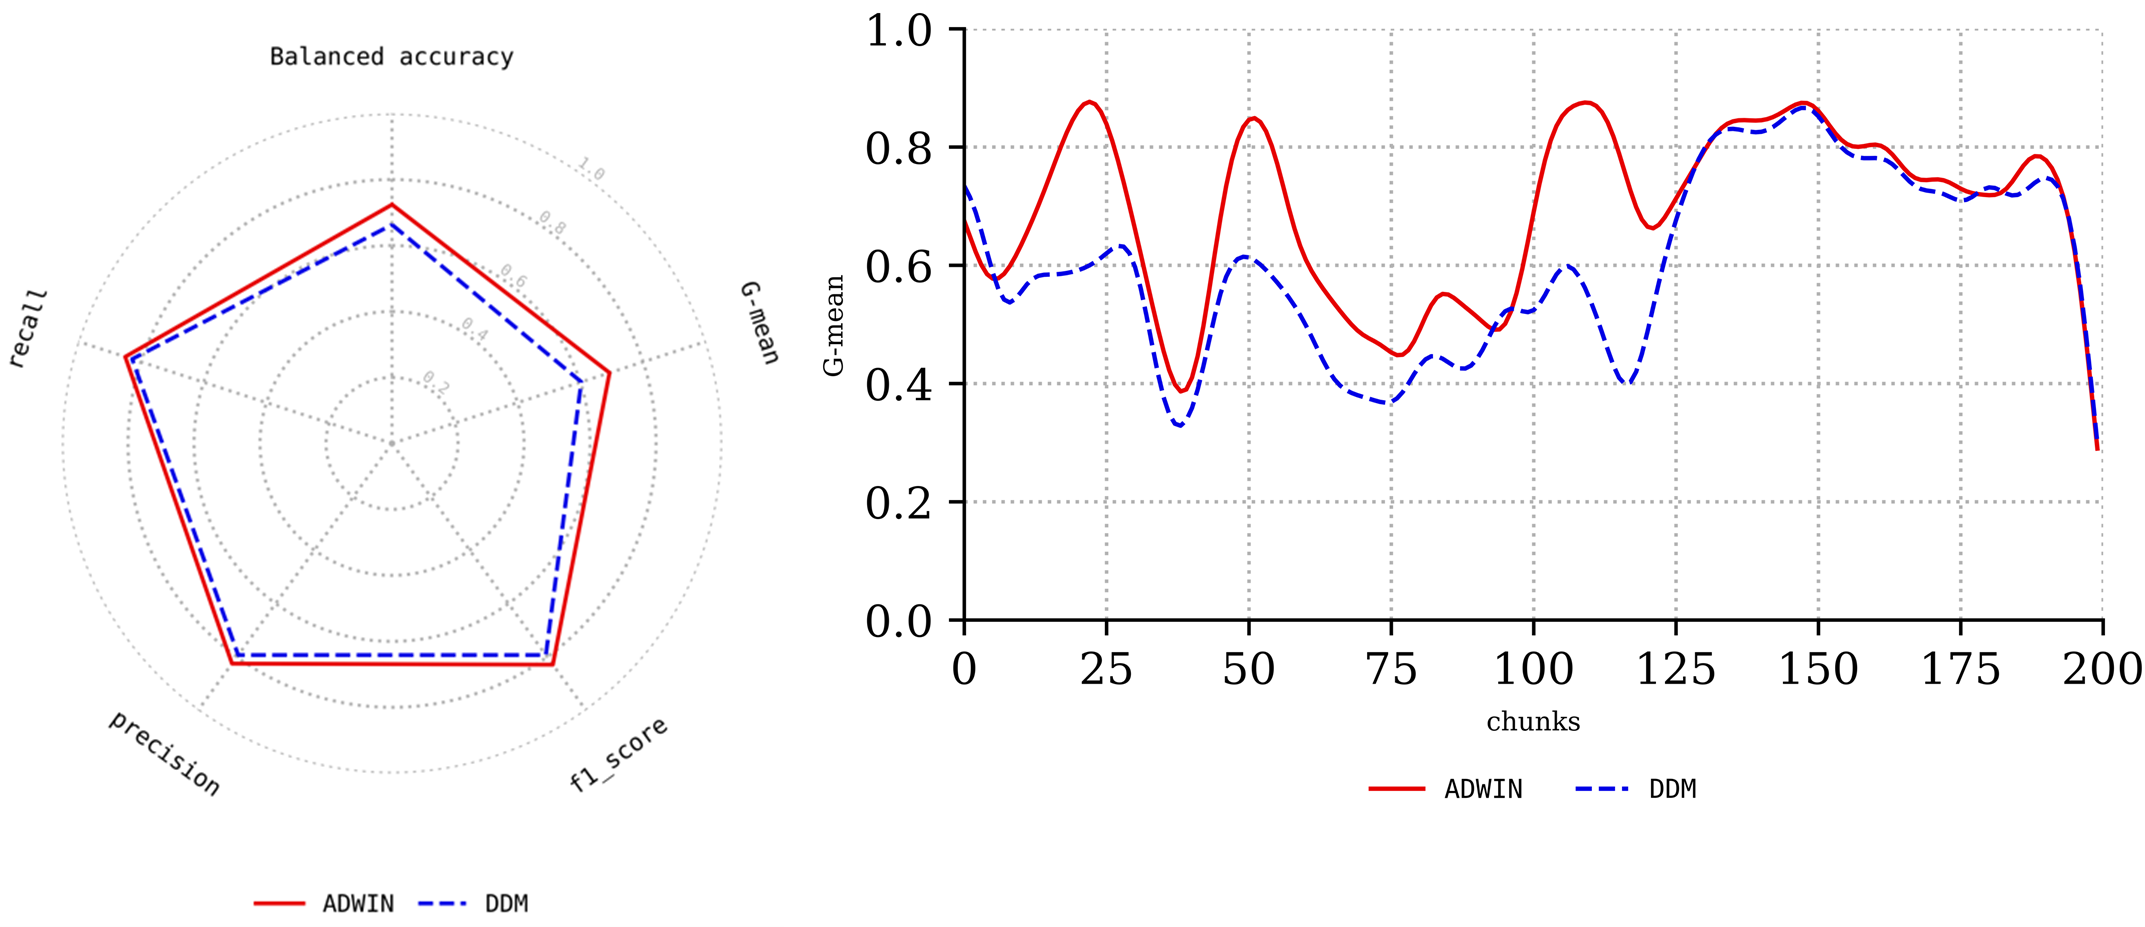
\includegraphics[width=1\linewidth]{5_Emerging/figures/result5}
    \end{figure}
 
    \begin{table}[h!]
      \centering
      \caption{Running time comparsion between ADWIN and DDM}
      \label{table:5_4}
      \begin{tabular}{|c|c|c|c|c|}
       
      \hline
      \textbf{Algorithm} & \textbf{KNN} & \textbf{SVC} & \textbf{GNB} & \textbf{HT} \\ \hline
      \textbf{Training Times} & 140 & 150 & 139 & 148 \\ \hline
      \textbf{Time (seconds)} & 586 & 878 & \textbf{291} & 1169 \\ \hline
      \end{tabular}
      \end{table}